\documentclass{article}
\usepackage[utf8]{inputenc}
\usepackage{graphicx}

\title{Assignment 7: Robotics Motion Planning}
\author{Avery Frankenberg}
\date{February 2019}

\begin{document}

\maketitle

\section{Motion Planning for Robot Arm}
\subsection{Introduction}
The goal for this first problem is to determine a way for a robot arm to move from one configuration to another while avoiding obstacles in the way. The robot arm can have 2, 3, or 4 segments that all rotate on a circular joint (i.e. can move 2pi radians or 360 degrees). To solve this problem we do the planning of motion not in the x, y plane but instead in the theta plane. This means that in our eventual planning from one configuration to another, we are determining the path by choosing different theta configurations and ensuring they are valid in the x,y space (i.e. they don't collide with obstacles). 

\subsection{Workspace}
For the first part of this assignment, the robot arm, I first had to create the kinematics of the robot arm, the graphical visualization of the arm and the obstacles, and the collision detection method associated with collisions in the workspace. All of these features are contained in the Workspace.py file. The workspace is initialized with a list of thetas of the initial representation, a list of the length of each arm, and a list of the obstacle locations and sizes. This class contains four additional methods. Calculate end points takes the theta values and the lengths and calculates the end locations of each of the segments of the robot arms. Calculate lines generates start and end points for each of the robot arms and puts this list of two tuples into a list of lines. The collided method checks if a given state, specified by the specific position of the robot arm segments, i.e. the lines, intersects any of the obstacles. If it does, then it returns True. If it doesn't it returns False. The final method in this class is the generate graphics method. This method plots the robot arm with all of its segments in different colors and the obstacles on the workspace which is a specified size. 

\subsection{Probabilistic Roadmap}
After generating the workspace for the problem layout the next task was to create and search via the Probabilistic Roadmap (PRM). This search is conducted in two step; the roadmap step and the query step. The roadmap can be used for many different queries, as long as the obstacles remain the same. The methods involved in the building of the roadmap are sampling, collision, local planner, k nearest neighbors manual, build roadmap, angular distance, and prm. The get edges and print prm method are only used to visualize the prm on the screen; however, this only works well for the arm with 2 links. 

The prm method is the main method called to do the probabilistic road map search. There is a boolena value that has to be passed in this method which indicates whether the manual K nearest neighbors search should be used or the scikit learn search. If the boolean is true it indicates that the manual one should be used (the scikit learn version is explained in the Bonus section). When this method is called, the build roadmap method is subsequently called. This method generates the roadmap by randomly sampling a combination of thetas, then calling the collision method to ensure the x,y configurations generated by these thetas do not intersect the obstacles. Next the local planner method is called to link this new point in the roadmap space to its k nearest neighbors. The k nearest neighbors are determined in the k nearest neighbors manual method where all of the points are looped over, the angular distance is calculated from the new point to each of the old points (in the angular distance method), and an ordered list is returned to the local planner method. The neighbors are only added to the list if they are close enough to the initial point, and as long as both points do not collide with an obstacle. In this way we can ensure that the path that the arm takes doesn't collide with any obstacles, even if it is not checking at every step along the way. The local planner then generates edges connecting the new point to its k nearest neighbors and adding these links to the edges list. 

After the roadmap is generated, the query part of the algorithm is run. In this part of the algorithm, the start and goal points are first added  to the roadmap by connecting them to the closest node using the local planner method. If they can successfully connect, then the roadmap is updated and the appropriate edges are also added to the edge list. Next, the astar method method is called. This method conducts the straightforward astar search on the roadmap graph that we have constructed. As we have turned the continuous theta space into a discrete graph of random points connected by k edges to other random points, this search will help us find the solution. 

Once a solution is found using the astar search, the backtrack method is called, which backtracks through and determines the solution path, overall cost, and number of nodes visited. The path is printed to the console, in addition the steps taken are added to the workspace graphic and the overall motion of the robot arm is printed as a final graphic. 

The following are testing images for 2, 3, and 4 arm segment robots. The line of the robot's arm gets lighter the more steps it takes, so you can tell when it has reached the final state as it is the lightest color in the image. 

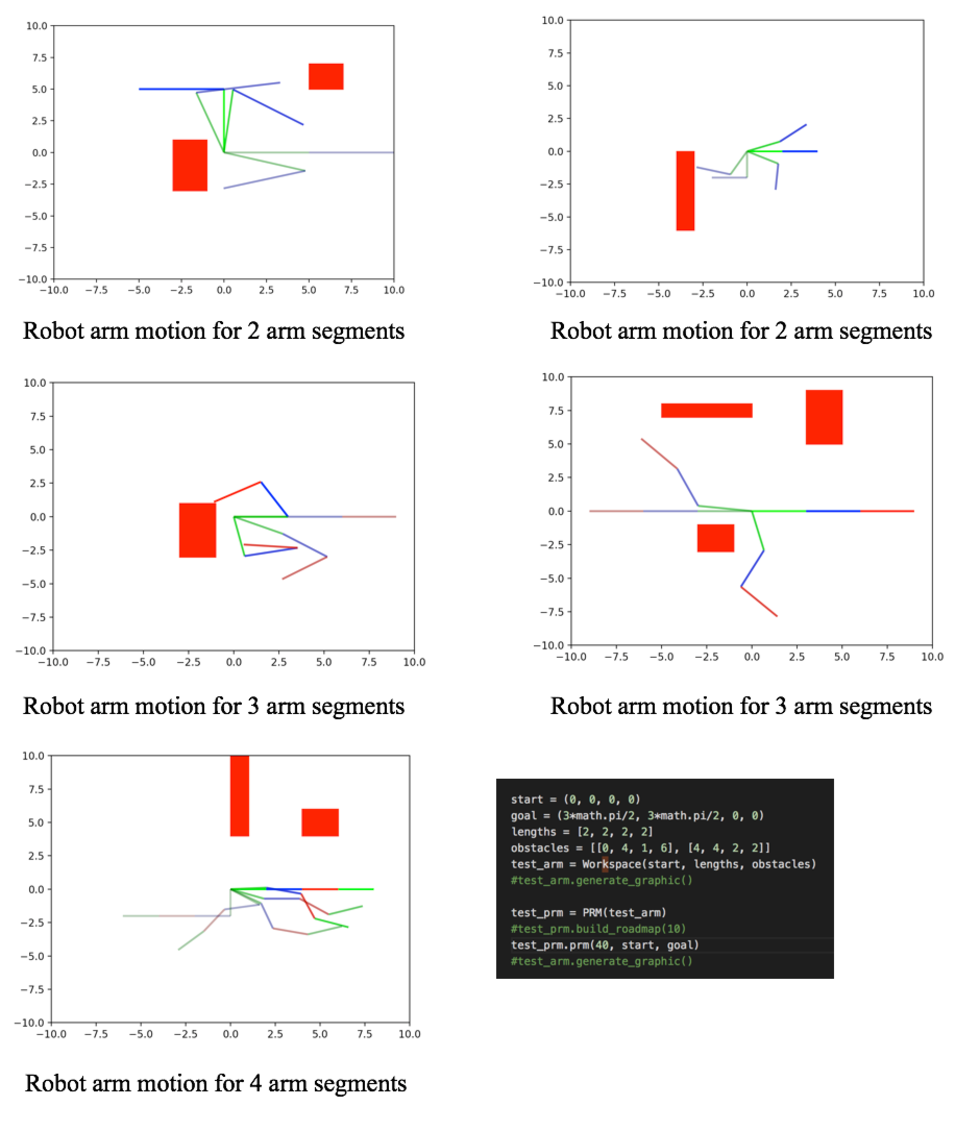
\includegraphics[width=\textwidth]{robot_2_3_4_arms.pdf}

In addition, here is an example of a PRM graph that is created for a 2 arm robot. This is plotted in the theta1, theta2 space and therefore the obstacles are not present but it demonstrates how random points are sampled in this space and then connected via edges. However, not every vertex is connected to every other vertex, which is appropriate because they should only be connected if they are close enough to one another. The graph is from 0 to a little larger than 6 as the theta values go from 0 to 2pi. In addition values close to 0 can be connected to values close to 6 becuase the space wraps around--this applies both on the x and y axis. 

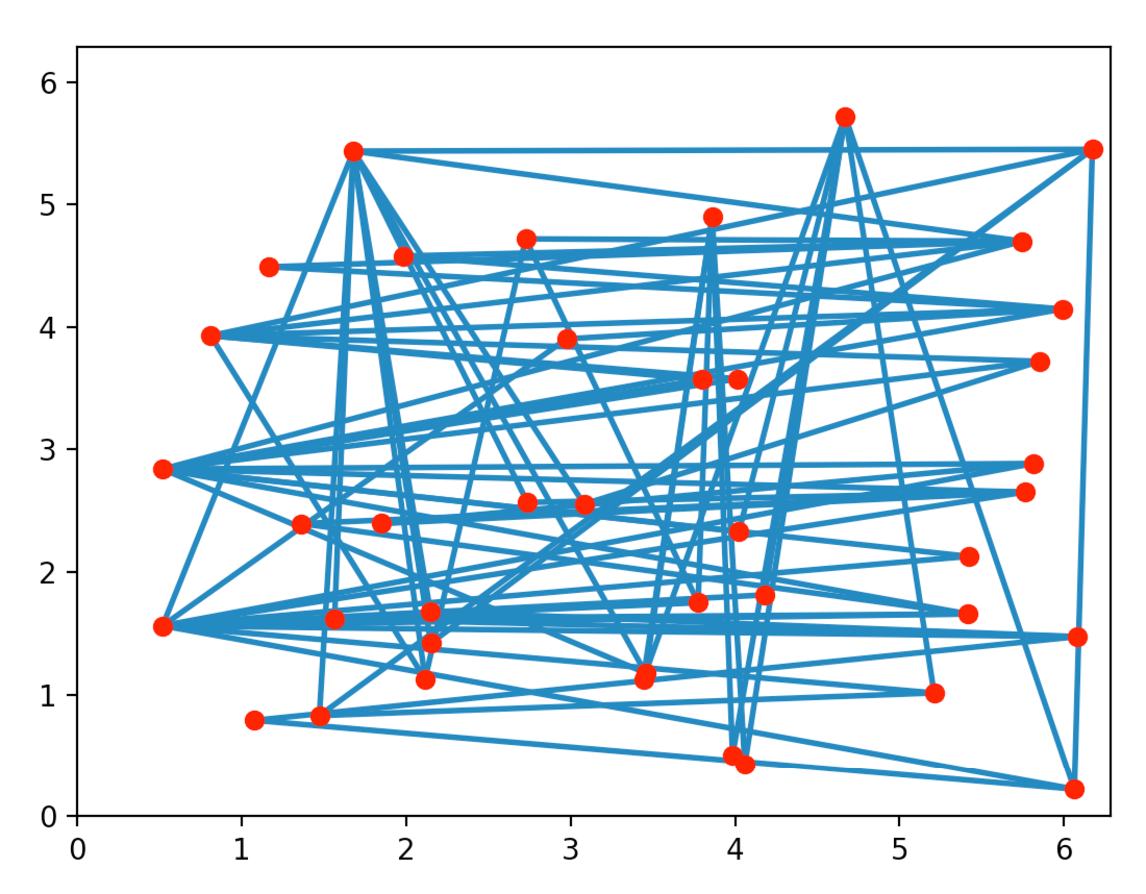
\includegraphics[width=\textwidth]{prm_example.pdf}

\section{Motion Planning for Robot Car}
\subsection{Introduction}
For this part of the project, I created algorithms to conduct motion planning for the robot car. Specifically we were to use the Rapidly Exploring Random Tree (RRT) algorithm. The workspace for this problem is the space (x, y, theta). In our implementation, the robot car can only move 6 different directions, forward, backward, forward turn left, forward turn right, backward turn left, and backward turn right. In the underlying implementation of the robot car motion these directions are implemented in a forward velocity and an angular velocity value. 

\subsection{Rapidly Exploring Random Tree}
To actually implement the RRT algorithm I expanded the rrt class. In the initialization of the rrt, four variables are passed in: start point, max distance, obstacles, and dist to goal. The start point is the initial (x, y, theta) value of the robot. The parent of this node is None as it is the root node. The max distance is the variable that dictates how close two states must be to say that the path between them doesn't collide with any obstacles if the two individual states don't collide with any obstacles. The obstacles variable contains a list of all of the obstacles in the space. The dist to goal variable determines how close to the goal the robot must be before it declares it has reached its target location. The rrt graph variable is also initialized in this method, it is an empty dictionary. 

The rrt complete method is the method running this algorithm. This method takes in two parameters, num vertices, which dictates how many points are generated in the (x, y, theta) space for the rrt, and goal which is the goal location for the search. It starts by passing these two parameters to the rrt alg method which runs the bulk of the algorithm. While in this loop a random point is generated (by calling the random point method). Then, using the local planner method, the neraest point on the current graph to this random point is determined--this is near point. Then the method simulates all 6 actions contained in controls rs. If the new point generated from each action does not collide with the obstacles, checked by running the collision method, then the can add edge method is called. This method returns True if the distance between near point and this next point is less than the maximum distance, otherwise it returns False. If it does return true, then the next point is added to the children list. In addition, this next point and the action used to reach this point is added to the state action dictionary. This will allow us to backchain the actions from given states when a goal state is found. After it is added to the children list, this point is checked to see if it is close enough to the goal to be considered successful. The distance dist to goal value is used to check if the next state generated is close enough to the goal. If it is not close enough to the goal, after all 6 actions are simulated, the near point is added to the rrt graph as a key with the corresponding value being a list of its children. If it is close enough, then the visualize rrt method is called which prints the rrt so that we can visualize the graph that was created. In addition, it calls the backchain method, obtaining the final path, and then returning this path to the rrt complete method. 

In the rrt complete method the finish rrt method is subsequently called by passing it the backchained final path. The path does not contain state locations, but instead it contains the index of the move necessary to get to a given state. After the path of actions is generated, the duration list is created which is a list of 2 second values for each action. I found through some experimenting that this generated the motion I liked best (one second wasn't enough time for each action to complete enough). Then the planar trajectory object is created and passed to the trajectory view object. After these two objects are created the trajectory view object is drawn and the rrt is complete. 

\subsection{Testing}

Below is an example of an RRT graph that is created, only with the (x, y) information of the robot car and subsequently the corresponding path that the robot car takes in space. We can see how the tree is growing, the growth was only terminated because a value close enough to the goal value was obtained and therefore the methods were called to obtain the path and have the robot car move appropriately.  

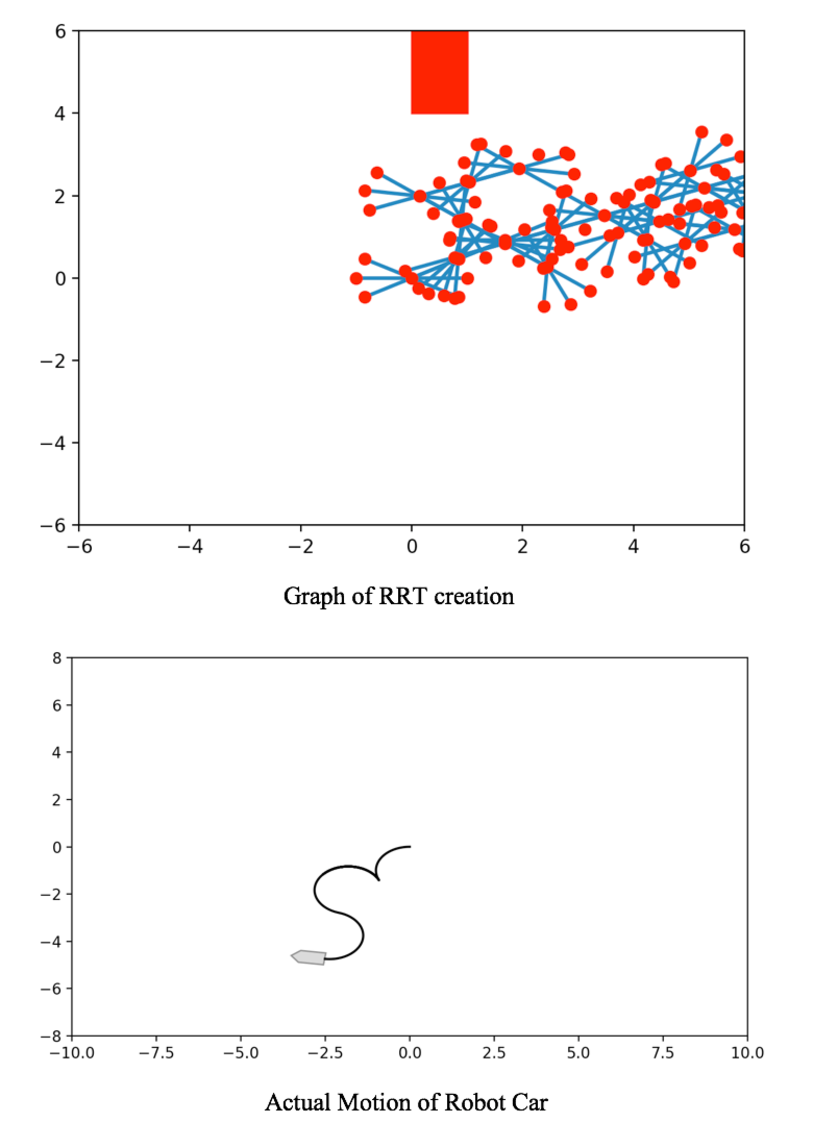
\includegraphics[width=\textwidth]{simple_rrt_example.pdf}

It is interesting to note how differently the RRT graphs are every time the algorithm is run. In addition, we can see how the graph spreads toward the goal differently depending on where it is. Below are some examples of different RRT graphs generated for two different goal locations (3, 3, 0) and (-3, -3, 0). 

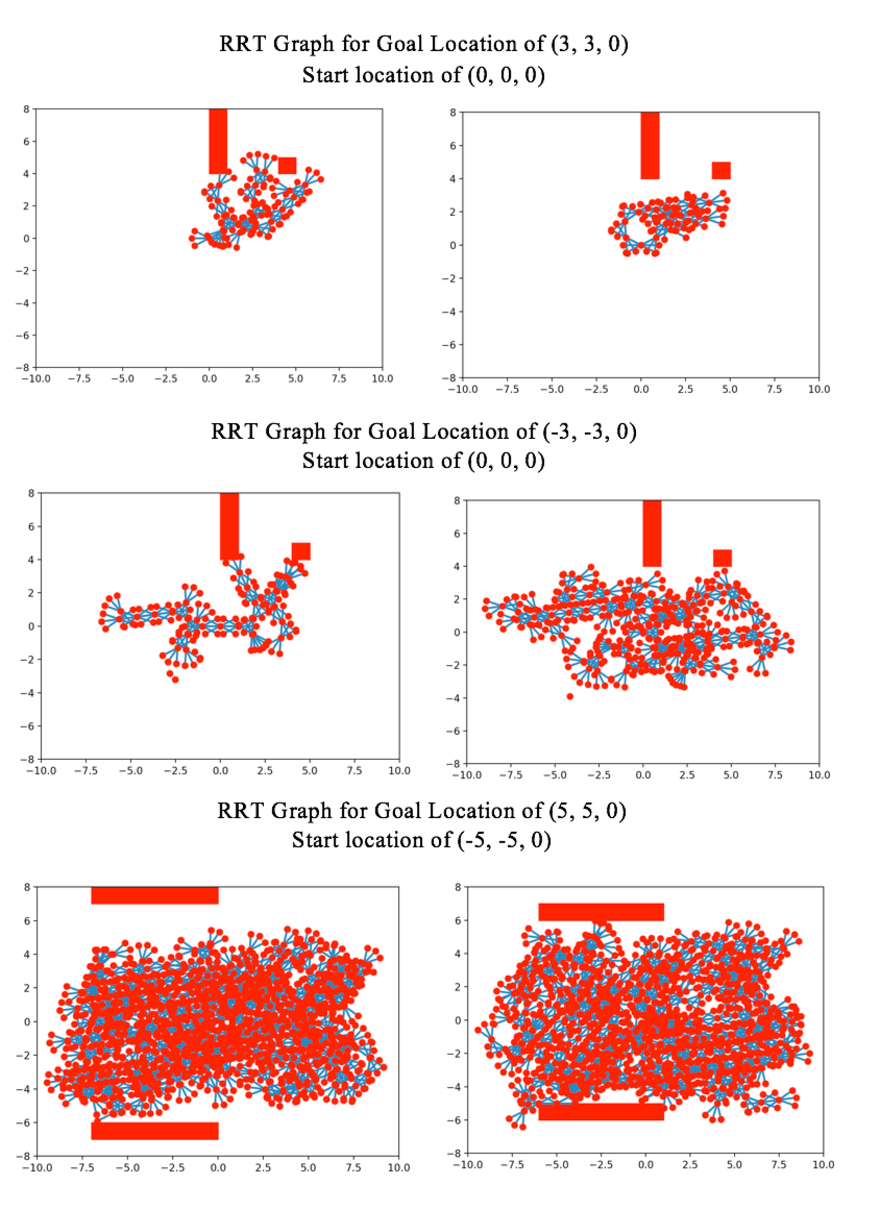
\includegraphics[width=\textwidth]{rrt_graph_examples.pdf}

Below is a solution to the hardest example present in the test RRT class. We can see how the motions aren't perfect and direct, but overall it is moving toward the goal location consistenlty and gets relatively close to it. In this case the start location was (-5, -5, 0) and the goal location was (5, 5, 0). In addition there were two obstacles in the field. 

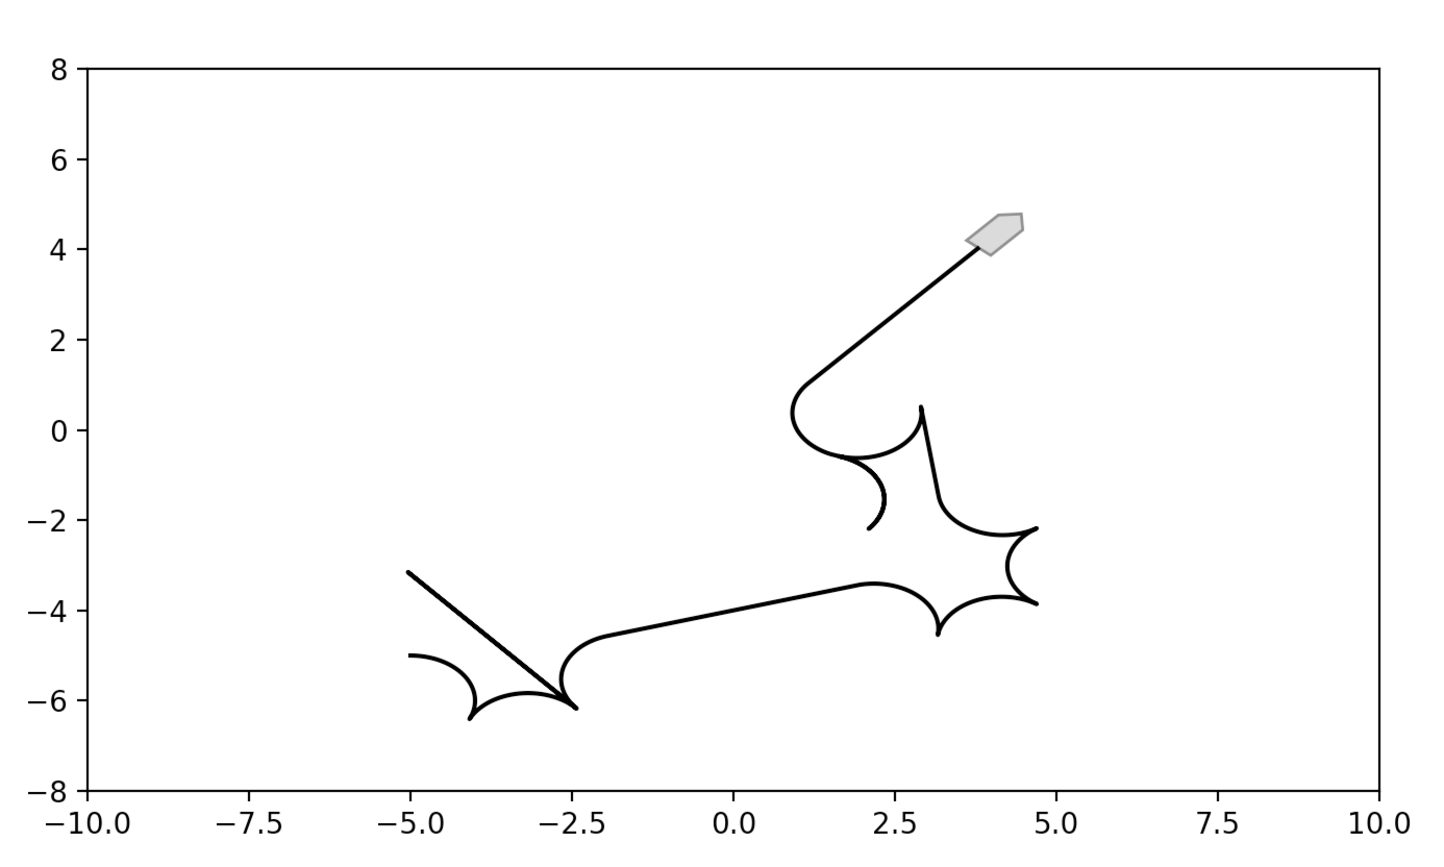
\includegraphics[width=\textwidth]{hard_test.pdf}
\section{Bonus}
\subsection{Previous Work: PRM}
To better understand extensions of PRM, I read an article called "Path Planning for Improved Visibility Using a Probabilistic Road Map" by Baummann et.al. This article explores the use of PRM techniques in an industrial setting where vision sensors are available but only work for a certain distance. The goal was to use this technique but to modify it in order to take advantage of the visual sensors--by maintaining visual contact with the target. To accomplish this goal the lab used two primary additions to the PRM algorithm: dynamic visibility checking and dynamic occlusion checking. The general PRM method works similarly; however, when an edge is added to the graph (that has been already checked for no collisions) it is added with an associated penalty. This penalty is proportional to the number of segments in the edge where the visibility of the target is obstructed. After this graph is generated with the penalties, they used Dijkstra's algorithm to calculate the lowest cost path from the start state to goal state.

I found this article particularly interesting because it demonstrates how this general PRM technique can be somewhat easily modified to take advantage of additional information. When implemented for robots with sensors, it seems to me that the inclusion of that information is extremely important. Therefore, the development of this PRM algorithm using vision sensors seems particularly beneficial and applicable. In the conclusion of the paper the authors describe how the algorithm can be improved by tailoring the penalty calculation. While this extension definitely seems helpful and necessary, the article overall inspired me to consider the inclusion of other sensory informaiton as well. Instead of only including penalties for vision obstruction it would be interesting to use other stimulus to inform the PRM algorithm (possible sound, touch/floor texture, etc) and help its overall performance.

\subsection{Previous Work: RRT}

To better understand applications of RRT, I read an article titled "Motion Planning for Steerable Needles in 3D Environments with Obstacles using Rapidly-Exploring Random Trees and Backchaining" by Xu et. al. This article describes the extension of RRT to direct needles in medical uses where the path the needle takes is extremely important and consequential for the patient. To determine possible locations for the needle tip in a given 3D space, they chose to used a modification on RRT to sample the space. The modification they made was instead of using deterministic sampling they used randomly sampled control space. In this initial paper the formulation they worked on was using only spherical obstacles and a rigid needle who's motion directly followed the motion of the bevel tip. They were able to create a model simulating motion planning for the needle, in this constrained space. For future work, this lab plans to modify the space and include different types of obstacles and more entry points. 

\subsection{K Nearest Neighbors}
As looping over all of the neighbors to determine the K nearest neighbors is very expensive, instead of doing this manually I created another method called k nearest neighbors which does this using the scikit learn NearestNeighbors method. This method is much more efficient at determining the nearest neighbors to a given theta point. It takes three parameters, the k value determining the number of neighbors the method should return, the theta, and the radius distance that specifies the distance between two points. 

If there are not more than k points in the roadmap already, then the method just returns the points that are already in the dictionary. However, if there are more than k points then the method creates a NearestNeighbors object with k neighbors as the n neighbors parameter, and the value of return distance as false. Then, the list of points (the keys of the roadmap), are fit to this nearest neighbor object. Afterward, the k neighbors method is called on this fit nearest neighbors object for the desired theta, and the indexes of the k nearest points are returned. Next, the samples are passed to the format samples method which returns them in the properly formatted list. Afterward, the points at the correct indices of the point list are appended to the neighbors list and returned to the local planner method. Then this local planner method continues on as normal to complete the prm. 

\subsection{Sources Used}

https://ieeexplore.ieee.org/abstract/document/8395123

https://ieeexplore.ieee.org/stamp/stamp.jsp?tp=&arnumber=5406221

\end{document}
